\documentclass[12pt]{article}
\usepackage{cite}
\usepackage{graphicx}
\usepackage[margin=1in]{geometry}
\usepackage{hyperref}
\usepackage[font={small,it}]{caption}
\usepackage{float}
\usepackage{setspace}
%\doublespacing

%\usepackage{lineno}
%\linenumbers

\hypersetup{
  colorlinks   = true,  %Colours links instead of ugly boxes
  urlcolor     = blue,  %Colour for external hyperlinks
  linkcolor    = black, %Colour of internal links
  citecolor   =  blue   %Colour of citations
}

\begin{document}
\title{Boosted Decision Trees for Machine Learning}
\author{Andrew Carnes}

\maketitle 

\newpage
\tableofcontents
\newpage

\section{Introduction}

This document outlines the Boosted Decision Tree (BDT) machine learning algorithm. The text here was originally written as part of a larger document for a project during my PhD at the Large Hadron Collider. I extracted the relevant BDT info and put it into this document in case people might find it useful. 

\section{Boosted Decision Trees}

Let's get to it. The BDT algorithm is a supervised machine learning algorithm: it learns from a set of data with known answers in order to predict data with unknown answers. The algorithm creates a forest, which is a collection of trees. The forest starts with a single tree, which chops up the feature space into discrete regions, fitting constants in each as to minimize the total error between between the true values and the predicted values of the tree. The function defining the net error is called the loss function. If the predictions by the tree are general enough the events (data points) will be off by some amount, i.e. the predicted values will still differ from the true values. Since the events are still off, the algorithm will add another tree attempting to correct the predictions of the last tree to further reduce the error. The algorithm will continue to add trees further correcting the predictions and minimizing the error until it reaches the maximum number of trees, a hyperparmeter set by the user.

\subsection{A Single Decision Tree}

The decision tree needs to decide how to partition the space such that it is computationally efficient and reduces the error defined by the loss function, $L(z,\hat{z})$, where $z$ is the vector of true values for all data points in the data set and $\hat{z}$ is the vector of predicted values. Usually $L(z,\hat{z})$ looks something like 
\begin{equation}
L(z,\hat{z}) = \sum_{j} l(z_j,\hat{z}_j)
\end{equation}
where $l(z_j,\hat{z}_j)$ denotes the loss (aka error) for a single data point with true value $z_j$ and predicted value $\hat{z}_j$. To meet the efficiency demand, the tree building algorithm takes a greedy approach, recursively dividng the regions into two until the maximum number of terminal nodes, a hyperparameter determined by the user, is reached. The maximum number of terminal nodes corresponds to the number of predictive regions in feature space. 

The algorithm goes as follows. First fit the entire feature space with the constant that minimizes the loss function in the entire space. Then for each feature, search for the best division among a set of candidate split values belonging to that feature. For each candidate value, propose a cut in the form of a hyperplane through a value of that feature, dividing the space into two candidate regions. Then fit the two candidate regions with the constants that minimize the loss in the respective regions. 

\begin{equation}
\frac{d}{dc_{R}} L(z,\hat{z} = c_{R}) = 0 \textrm{ | } z,\hat{z} \in R
\end{equation}

The loss before the subdivision, $L_{before} = L(z,\hat{z}_{before})$, is compared to the loss after the subdivision, $L_{after} = L(z,\hat{z}_{after})$, and the error reduction is calculated like so, $-(L_{after} - L_{before})$, which is a positive number since $L_{after}$ has a smaller error than $L_{before}$. Call $R_{i}$ the region to split and $R_{i,1}$ and $R_{i,2}$ the resulting regions after the proposed split. Again using $l(z_j,\hat{z}_j)$ to denote the loss for a single data point with true value $z_j$ and predicted value $\hat{z}_j$ then the error reduction may be written, 

\begin{equation}
\textrm{Error Reduction} = \sum_{j \in R_{i}} l(z_j,c_i) - \sum_{j \in R_{i,1}} l(z_j,c_{i,1}) - \sum_{j \in R_{i,2}} l(z_j,c_{i,2}).
\end{equation}

The cut with the largest error reduction of those searched is the best cut for the feature. The algorithm checks the other features in the same manner, reporting the best cut and error reduction for each. The cut chosen for the region is the cut with the largest error reduction of all the features. Now the feature space is divided into two regions, each with constant fits. The algorithm then repeats the same process in each subregion, figuring out the best cut and constants for each, eventually splitting the region that provides the maximum gain in error reduction. This process continues, each time splitting the subspace that yields the best return, until the number of regions equals the maximum number of terminal nodes set by the user. 

\subsection{Building a Single Decision Tree: an Example}

Here is an example of the tree building algorithm using Least Squares as the loss function. Consider a case with N events where each event has two features x and y, and each event is uniquely labeled by the subscript i. The maximum number of terminal nodes in this example is 3.

\begin{equation}
\textrm{Least Squares} \equiv \frac{1}{2}\sum_{i=1}^{N} [z(x_i,y_i)-\hat{z}(x_i,y_i)]^2
\end{equation}

\begin{equation}
\frac{d}{dc_R}\frac{1}{2}\sum_{i=1}^{N} [z(x_i,y_i)-c_R]^2 = 0 \rightarrow c_R = \frac{1}{N}\sum_{i=1}^{N}z_i
\end{equation}

Take a look at the the top left of Figure \ref{fig:dtbuild}. The events for the example were generated such that those with x$>$0.5 have a true value z=10, those with x$<$0.5 and y$>$0.5 have z=-8, and those with x$<$0.5 and y$<$0.5 have z=-12. The colored regions represent the true values of the underlying true distribution and the crosses represent the generated events themselves. In the end the tree with three terminal nodes should model these generated regions, correctly predicting the events. In the next three pictures in Figure \ref{fig:dtbuild} the colors of the crosses still represent the true values, but the colored regions represent the fits in the decision tree regions at each iteration.

\begin{figure}[h!]
  \centering
  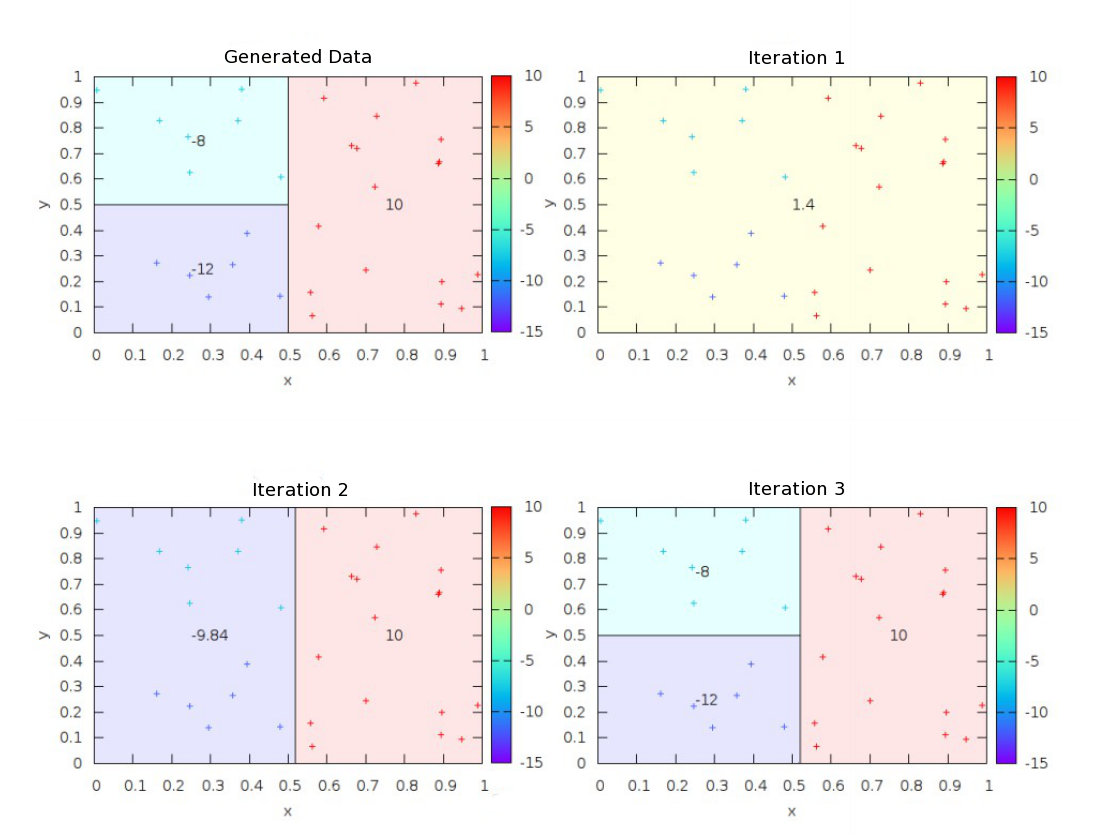
\includegraphics[width=6in]{imgs/BDT_featurespace_iteration.png}
  \caption
   {The stages of creation for a single decision tree with three terminal nodes.}
  \label{fig:dtbuild}
\end{figure}

\newpage

Equation 3 determines that the constant fit in a region should be the mean of the true values in the region. So in iteration 1 the tree fits all of the events with the mean, 1.4. Then in iteration 2 the tree searches along x and y calculating the error reduction for each possible cut along each feature. The cut with the maximum error reduction turns out to be x=0.535. The left region is fit with its mean, -9.84 and the right region with its mean, 10. The tree then searches in both subspaces along x and y for the best split in each space, choosing to split the region with the most gain. The algorithm finds the maximum error reduction in the left region with a cut at y=0.5, fitting the top with -8 and the bottom with -12. At the end of iteration 3 there are three terminal nodes and the algorithm stops building the tree. The tree has correctly modeled the underlying distribution of the true values. 

Notice that the fit for an event is a given by a series of binary decisions, and that the entire model is given by a tree of binary decisions, hence the name. The tree structure is illustrated for the previous example in Figure \ref{fig:dtstruct}.

\begin{figure}[h!]
  \centering
  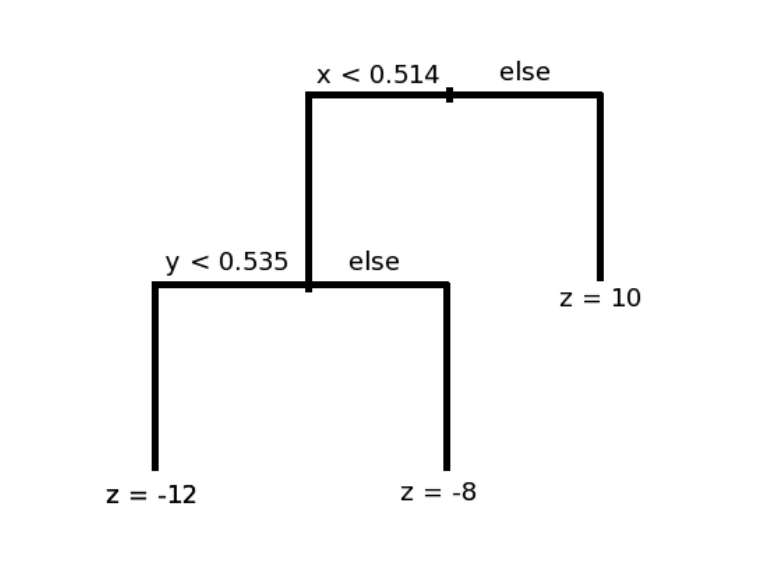
\includegraphics[width=4in]{imgs/BDT_tree_structure.png}
  \caption
   {The decision tree model gets its name from the fact that it can be viewed as a tree of binary decisions.}
  \label{fig:dtstruct}
\end{figure}

\newpage
\subsection{The Decision Tree Algorithm}

Now that the basic concepts behind the decision tree have been covered, the decision tree algorithm is outlined in pseudocode.

\begin{verbatim}

node                 |  tree
  bestSplitValue     |    rootNode
  bestSplitFeature   |    terminalNodes
  bestErrorReduction |    trainingEvents
  fitValue           |    loss_function
                     |    nodeLimit
  mother             |    
  leftDaughter       |
  rightDaughter      |
                     |
  loss_function      |

node::fitAndCalcOptimumSplit(loss_function)
# General outlining the necessary steps to calculate
# the best split value, feature, and error reduction
# for the node

  bestSplitValue = 0
  bestSplitFeature = -1
  bestErrorReduction = -1

  # get the constant fit value in this region aka subspace aka node
  # based upon the constant that minimizes the loss function
  fitValue = loss_function.fit_constant(events)

  # calculate the error reduction for each feature
  # and for a set of points along that feature
  # store the information for the best one
  for(f in features)
      for(splitPoint in f)
          errorReduction = loss_function.calculateErrorReduction(events, splitPoint, f)
          if(errorReduction > bestErrorReduction)
            bestErrorReduction = errorReduction
            bestSplitFeature = f
            bestSplitValue = splitPoint

tree::buildTree()
# build a tree up to the given node limit

  # set up the root node for the tree
  rootNode = new node
  rootNode.events = trainingEvents
  terminalNodes.add(rootNode)

  # keep track of the node with the best error reduction
  # during the loop through the nodes
  bestNodeErrorReduction = -1
  nodeToSplit = 0

  # set fit value and figure out the best split
  # feature, split value, and best error reduction
  # for the root node
  if(terminalNodes.size() == 1)
    rootNode.fitAndCalcOptimumSplit(loss_function)

  # All terminal nodes have best split info available
  # see which one is the best one to split
  for(node in terminalNodes)
    if(node.bestErrorReduction < bestNodeErrorReduction)
      bestNodeErrorReduction = node.bestErrorReduction
      nodeToSplit = node

  # found best terminal node aka subspace to split
  # link mother and daughter nodes
  left = new node
  right = new node
  nodeToSplit.leftDaughter = left
  nodeToSplit.rightDaughter = right
  left.mother = nodeToSplit
  right.mother = nodeToSplit

  # filter the events appropriately from the mother space into the subspaces
  for(event in nodeToSplit.events)
    if(event.feature[nodeToSplit.bestSplitFeature] < nodeToSplit.bestSplitValue)
      left.events.append(event)
    else 
      right.events.append(event)

  # calculate the best split info for the new nodes
  # also figure out the constant fits for each region
  left.fitAndCalcOptimumSplit(loss_function)
  right.fitAndCalcOptimumSplit(loss_function)

  # nodeToSplit has been divided into subspaces
  # it is no longer a terminal node, but the daughters are
  terminalNodes.remove(nodeToSplit)
  terminalNodes.add(left)
  terminalNodes.add(right)

  # continue greedily dividing until nodeLimit is reached
  if(terminalNodes.size() < nodeLimit) buildTree()

\end{verbatim}

\subsection{Boosting}

Boosting involves iteratively adding trees to create a forest. Each subseuqent tree corrects the predictions of the earlier trees. 

\begin{equation}
\textrm{Forest}(\vec{x}) = T_0(\vec{x}) + T_1(\vec{x}) + ... + T_n(\vec{x})
\end{equation}

Now $T_0$ is the initial fit and fits the true values as well as possible. Then, $T_1$ is created such that it corrects the predictions of $T_0$. After, $T_2$ corrects $T_0 + T_1$, and in general the n$^{th}$ tree, $T_n$, corrects the predictions given by the previous n trees. This is analogous to perturbation theory in physics. The values the n$^{th}$ tree should model at each iteration are given by $d\hat{z}_{n}$ such that this correction heads in the direction of the minimum at that stage. This implies that $d\hat{z}_{n}$ should be in the same direction as the negative of the gradient, and that the nth corrective term to the forest, $T_n$, should model $d\hat{z}_{n}$ up to some constant.

\begin{equation}
-\frac{d}{d\hat{z}_{n-1}(x^i)}L(z(x^i),\hat{z}_{n-1}(x^i) = T_0(x^i)+...+T_{n-1}(x^i)) \rightarrow d\hat{z}^{i}_{n}
\end{equation}

In this way, the n$^{th}$ tree is an additive correction fit to the desired corrections, $d\hat{z}^{i}_{n}$. In other words, the tree chooses the appropriate splits and constants using the $d\hat{z}^{i}_{n}$'s as the true values. Because computationally efficient methods exist for building a tree with Least Squares, most implementations fit fit the n$^{th}$ targets for the specific loss function using Least Squares rather than the loss function itself. Fitting the appropriate corrections guarantees that the algorithm heads downhill, but further steps can be taken to reach a more minimum value. After the tree has modeled the gradient by forming the regions in feature spaceand fitting them with constants, the constants in those regions can be recalculated as to best minimize the loss function within each region. 

\begin{equation}
\frac{d}{dc_{n,R}} L(z,\hat{z} = T_0 + T_1 + ... + T_{n-1} + c_{n,R}) = 0 \rightarrow c_{n,R}
\end{equation}

If the user wishes to head downhill slower or quicker the user can supply a learning rate value, which scales each tree's predictions by a constant. If the learning rate were 0.3 then the constant fits in each of the terminal regions would be scaled by 0.3 for every tree. Trees are added until the number of trees in the forest reaches the maximum number of trees specified by the user as a hyperparameter.


\subsection{The BDT Algorithm}

Now that the concepts behind the decision tree and boosting have been covered, the BDT algorithm is outlined in pseudocode.

\begin{verbatim}

forest
  trainingEvents
  trees
  loss_function

  nodeLimit
  treeLimit
  learningRate

forest::buildForest()

  while(trees.size() < treeLimit)
    # head downhill by setting the targets for the tree
    # the target is the gradient for the loss function
    # covered earlier, each tree fits the targets as if
    # they were the true values
    for(event in trainingEvents)
      loss_function.set_target(event)  

    # build the tree
    # the tree usually uses least_squares to fit the targets
    # since it's efficient
    tree = new tree
    trees.add(tree)
    tree.buildTree(nodeLimit)

    # Now recalculate the best fits in the terminal regions
    for(tnode in tree.terminalNodes)

      # constant that minimizes the loss function in the region
      tnode.fitValue = loss_function.fit_constant(tnode.events)

      # scale by learningRate, hyperparameter set by user
      tnode.fitValue*=learningRate
  
      # update the predictedValue now that the event has 
      # been fit by a new tree
      for(event in tnode.events)
          event.predictedValue+=tnode.fitValue

\end{verbatim}

\subsection{Some Loss Functions}
Different loss functions create different trees depending upon the events the loss function focuses on. Having different options for the loss functions allows the user to focus on the events they care about and predict those more accurately. Least Squares, Huber, and Absolute Deviation are some common options for regression. I may add cross entropy to cover (multi)classification, but the writeup I extracted this text from was written for a regression project, so that's not covered at the moment. 

Anyways, let's cover the implemention and functionality of some common error metrics. Relative to Least Squares, Huber focuses on the core of the residuals, those events with small $|z-\hat{z}|$ values, while comparatively discounting events with large $|z-\hat{z}|$ values. Absolute deviation focuses even more than Huber on the events in the core, small $|z-\hat{z}|$. Depending on their goals, the user may want to focus on the hard to predict events and reign them in or they may want to ignore very difficult events in favor of more accurate predictions for the easier events. 

\subsubsection{LossFunctionBDT}

LossFunctionBDT is the interface. All of the methods require implementation when inherited. The fit is the constant that minimizes the loss function for the events in the node. The target is the target for the upcoming tree in the forest to model. It is the negative gradient of the loss function with respect to the predicted value for an event. Init must initialize the parameters for the loss function if they exist and provide the events with an initial fit.  

\begin{verbatim}
class LossFunctionBDT
  virtual Init(events)                  # initialize the loss function
  virtual SetTargets(events)            # set targets for collection of events
  virtual Target(event)                 # set target for one event
  virtual Fit(events)                   # set fit for collection of events in a node
\end{verbatim}

\subsubsection{LeastSquaresLossFunctionBDT}

This loss function implements LossFunctionBDT and defines the appropriate behavior for the Least Squares error metric.

\begin{equation}
\textrm{Least Squares} \equiv \frac{1}{2}\sum_{i=1}^{N} [z^i-\hat{z^i}]^2
\end{equation}

Taking a derivative with respect to the i$^{th}$ predicted value yields the residual. Setting $\hat{z}$ to a constant for all i and taking a derivative with repect to $\hat{z}$ yields the constant of best fit, the mean of the residuals.    

\begin{verbatim}
class LeastSquaresLossFunctionBDT
  Init(events)  # set initial predictions to the mean
    mean = Fit(events)
    for(event in events)
      event.predictedValue+=mean

  SetTargets(events)  
    for(event in events)  
      event.target = Target(event)

  Target(event)  # residual                 
    return event.trueValue - event.predictedValue

  Fit(events)    # mean                 
    mean = 0
    for(event in events)
      mean+=event.trueValue-event.predictedValue
    mean=mean/events.size()
    return mean;

\end{verbatim}

\subsubsection{AbsoluteDeviationLossFunctionBDT}

This loss function implements LossFunctionBDT and defines the appropriate behavior for the Absolute Deviation error metric.

\begin{equation}
\textrm{Absolute Deviation} \equiv \sum_{i=1}^{N} |z^i-\hat{z^i}|
\end{equation}

Taking a derivative with respect to the i$^{th}$ predicted value yields +1 for $z>\hat{z}$ and -1 for $z<\hat{z}$. Setting $\hat{z}$ to a constant for all i and taking a derivative with repect to $\hat{z}$ yields the constant of best fit, the median of the residuals.    

\begin{verbatim}
class AbsoluteDeviationLossFunctionBDT
  Init(events)  # set initial predictions to the median
    median = Fit(events)
    for(event in events)
      event.predictedValue+=median

  SetTargets(events)  
    for(event in events)  
      event.target = Target(event)

  Target(event)  # sign of residual                 
    return sign(event.trueValue - event.predictedValue)

  Fit(events)    # median                
    for(event in events)
      residuals.add(event.trueValue-event.predictedValue)
    return median(residuals);

\end{verbatim}

\subsubsection{HuberLossFunctionBDT}

This loss function implements LossFunctionBDT with the appropriate behavior for the Huber error metric. Huber has one parameter, the quantile defining the cutoff residual, $\delta$. The quantile parameter and the distribution of the events' residuals determine $\delta$. For a quantile of 0.7, $\delta$ would be $|z-\hat{z}|$ where 70\% have a $|z-\hat{z}|$ value less than or equal to $\delta$.

\begin{equation}
\textrm{Huber} \equiv \sum_{i=1}^{N} f(z^i, \hat{z}^i; \delta)
\end{equation}

$$
f(z,\hat{z}; \delta) = \left\{
        \begin{array}{ll}
            \frac{1}{2}(z-\hat{z})^2 & \quad |z-\hat{z}| \leq \delta \\
            \delta|z-\hat{z}| - \frac{1}{2}\delta^2 & \quad otherwise
        \end{array}
    \right.
$$

Taking a derivative with respect to the i$^{th}$ predicted value yields sign($z-\hat{z}$)min($|z-\hat{z}|$,$\delta$). Setting $\hat{z}$ to a constant for all i and taking a derivative with repect to $\hat{z}$ yields the constant of best fit, the shifted median. The shifted median is between the mean and the median. The exact form is shown in the code below. As the quantile of the cutoff goes to 100\% the shifted median approaches the mean. As the quantile goes to 0\% the shifted median approaches the median. So Huber can be tought of as a mixture of Least Squares and Absolute Deviation, where the quantile determines the mixing. 

\begin{verbatim}
class HuberLossFunctionBDT

  fQuantile        # set by user
  fResidualCutoff  # delta

  Init(events)  # set initial predictions to the shifted_median
    shifted_median = Fit(events)
    for(event in events)
      event.predictedValue+=shifted_median

  SetTargets(events)  
    for(event in events)  
      event.target = Target(event)

  Target(event)  # sign of residual                 
    residual = event.trueValue - event.predictedValue
    return sign(residual)*min(fResidualCutoff, abs(residual))

  Fit(events)    # shifted_median                
    residualMedian = getResidualMedian(events)
    shift = 0
    for(event in events)
      residual = event.trueValue - event.predictedValue
      diff = residual-residualMedian
      # shift will be average of differences from median
      # except that we discount diff to the residual cutoff
      # if it is too large.
      shift+=1/events.size()*sign(diff)*min(fResidualCutoff,abs(diff))
    return (residualMedian + shift)

\end{verbatim}

\section{Conclusion}

The End.

\begin{thebibliography}{9}
\bibitem{friedman} 
Friedman, Jerome H. “Greedy Function Approximation: A Gradient Boosting Machine.” The Annals of Statistics, vol. 29, no. 5, 2001, pp. 1189–1232. www.jstor.org/stable/2699986.
\bibitem{statlearn} 
Trevor Hastie, Robert Tibshirani, Jerome Friedman. The Elements of Statistical Learning: Data Mining, Inference, and Prediction. 2009. https://statweb.stanford.edu/~tibs/ElemStatLearn/ 
\end{thebibliography}
\end{document}
